\begin{figure*}[t]
\begin{subfigure}{0.3\textwidth}
   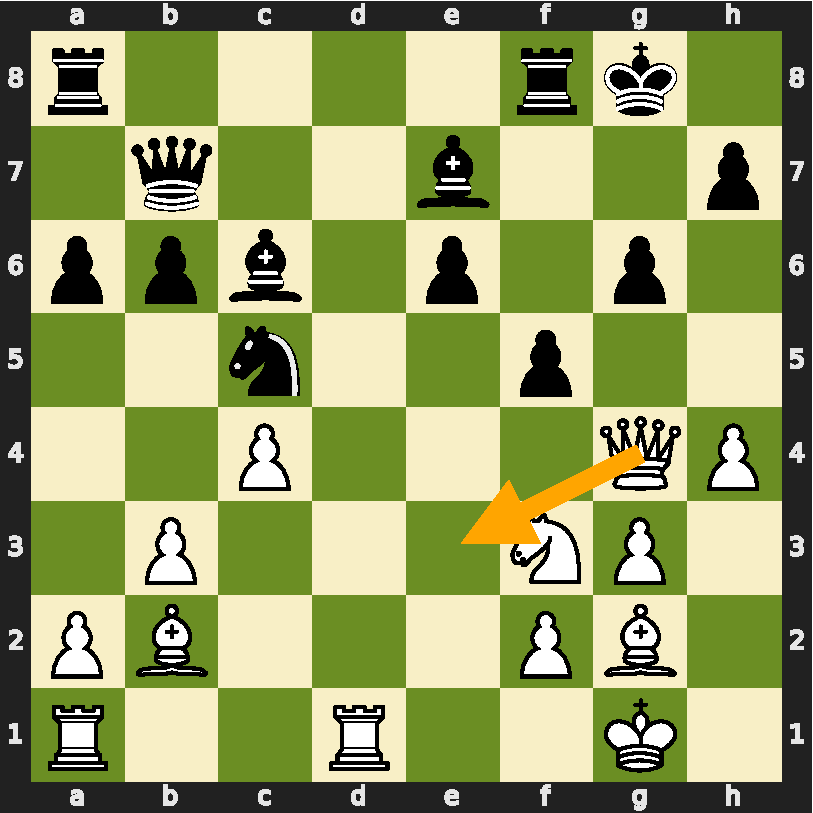
\includegraphics[width=\linewidth]{figures/board_syntax.pdf}
   \caption{\emph{Syntax}: Queen can move like all other piece types except for knight.} \label{fig:error_syntax}
\end{subfigure}
\hspace*{\fill}
\begin{subfigure}{0.3\textwidth}
   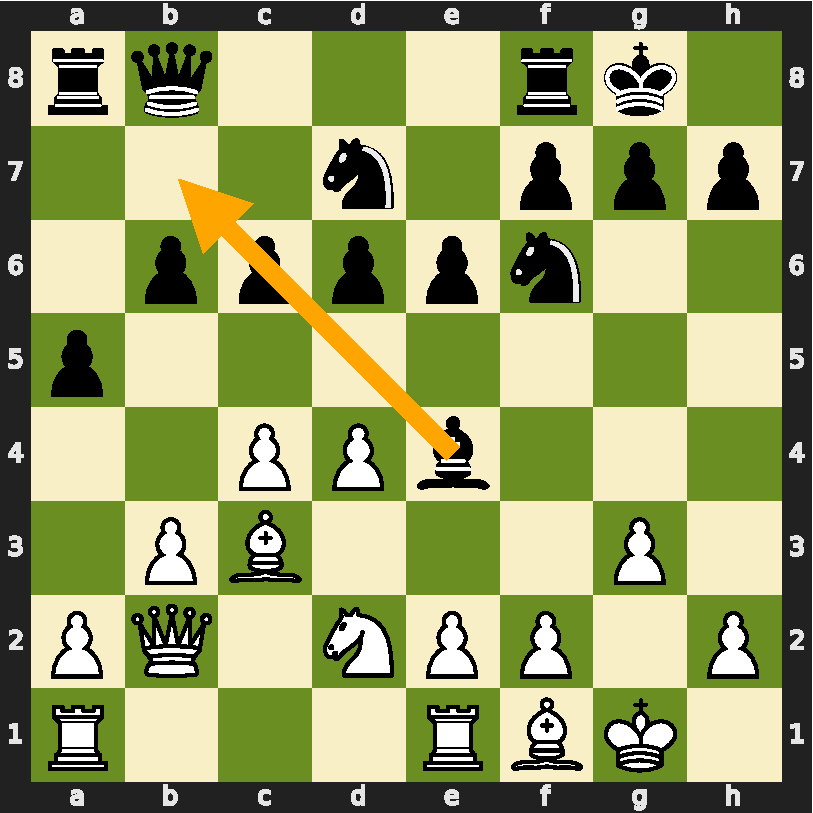
\includegraphics[width=\linewidth]{figures/board_path.pdf}
   \caption{\emph{Path Obstruction}: The pawn at \pos{c6} is blocking the bishop.} \label{fig:error_path}
\end{subfigure}
\hspace*{\fill}
\begin{subfigure}{0.3\textwidth}
   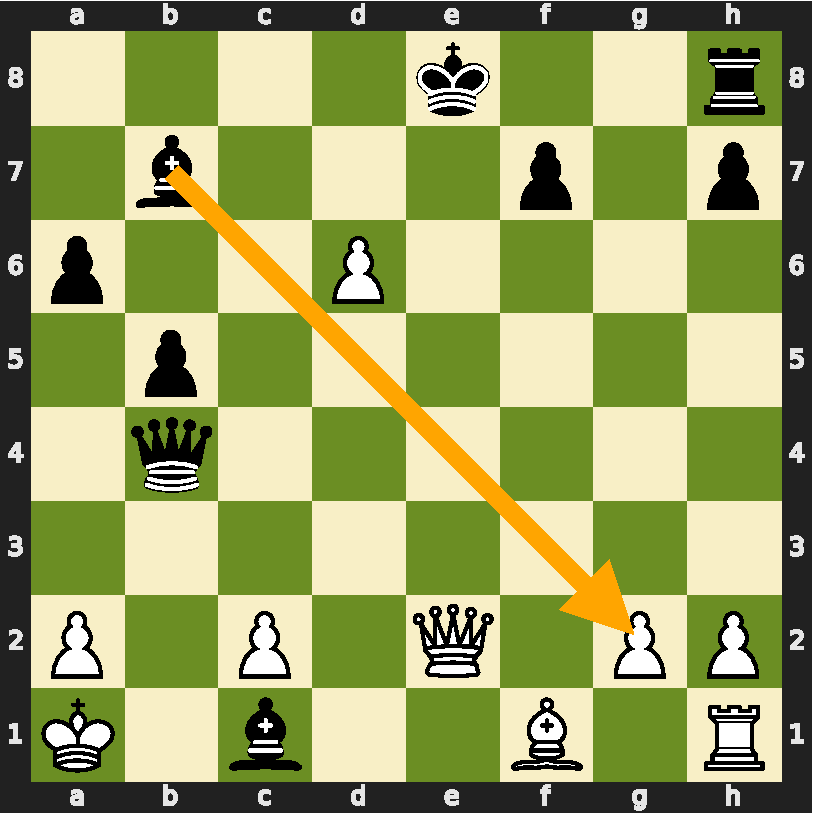
\includegraphics[width=\linewidth]{figures/board_pseudo.pdf}
   \caption{\emph{Pseudo Legal}: The black king remains in check.} \label{fig:error_pseudo}
\end{subfigure}
\caption{Instances of the three prominent categories of illegal ending square predictions.}
\label{fig:error_categories}
\end{figure*}
